\documentclass[12pt]{article}

\usepackage{sbc-template}
\usepackage{graphicx,url}
\usepackage[utf8]{inputenc}
\usepackage[brazil]{babel}
\usepackage{amsmath}
\usepackage{booktabs}
\usepackage{multirow}
\usepackage{algpseudocode}
\usepackage{float}
\newfloat{algoritmo}{htp}{loa}
\floatname{algoritmo}{Algoritmo}

\titlespacing*{\section}{0pt}{0.2ex}{-0.3ex}
\titlespacing*{\subsection}{0pt}{0.2ex}{-0.3ex}
\linespread{0.78}

\sloppy

\setlength{\textfloatsep}{2pt plus 1pt minus 2pt}
\setlength{\floatsep}{2pt plus 1pt minus 1pt}
\setlength{\intextsep}{2pt plus 1pt minus 1pt}

\setlength{\abovedisplayskip}{3pt plus 1pt minus 1pt}
\setlength{\belowdisplayskip}{3pt plus 1pt minus 1pt}
\setlength{\abovedisplayshortskip}{2pt plus 1pt minus 1pt}
\setlength{\belowdisplayshortskip}{2pt plus 1pt minus 1pt}

\title{Solver Pentadiagonal Híbrido CPU--GPU com Ajuste Dinâmico por
Simulated Annealing para o Benchmark NPB SP}

\author{André Gualberto\inst{1}, Gabriel Thomaz do Nascimento\inst{1}}

\address{Laboratório Nacional de Computação Científica (LNCC)\\
  Av. Getúlio Vargas, 333 -- 25651-075 -- Petrópolis -- RJ -- Brasil
  \email{agualber@lncc.br, thomazgb@lncc.br}
}

\begin{document}

\maketitle

\begin{abstract}
  The scalar pentadiagonal solver of the NAS Parallel Benchmark (NPB SP)
  is a memory- and latency-bound workload in which GPUs typically achieve
  modest speedups. This work presents a hybrid CPU--GPU implementation of
  the pentadiagonal sweep in which the fraction of lines assigned to each
  processing unit is adjusted at runtime by a simulated annealing (SA)
  heuristic that minimizes the measured time of each sweep window. The
  implementation was validated for reproducibility by bit-identical
  checksums across 1000 iterations, and executed with thermal monitoring
  via NVML. On an NVIDIA RTX 5000 Ada, the hybrid solver solved
  1.061,191,680,000 points (1.061 trillion) as 1,040,384,000 linear systems
  of order 1020 in 213.9~s, at 163~ms per sweep and 182 GFLOPS (28
  flops/point estimate), surpassing both the pure-GPU (185~ms) and pure-CPU
  (611~ms) modes. The same adaptive scheme reached 4.86 million pentadiagonal
  systems per second, in the same order as the NPB-GPU CUDA reference (200--216
  GFLOPS, NAS official counting) on the same hardware.
\end{abstract}

\begin{resumo}
  O solver pentadiagonal escalar do benchmark NAS Parallel Benchmark (NPB SP)
  é uma carga de trabalho limitada por memória e latência, na qual GPUs
  tipicamente atingem acelerações modestas. Este trabalho apresenta uma
  implementação híbrida CPU--GPU da varredura pentadiagonal em que a fração
  de linhas atribuída a cada unidade de processamento é ajustada em tempo de
  execução por uma heurística de simulated annealing (SA) que minimiza o
  tempo medido de cada janela de varredura. A implementação foi validada
  quanto à reprodutibilidade por checksums bit-idênticos ao longo de 1000
  iterações e executada com monitoramento térmico via NVML. Em uma NVIDIA
  RTX 5000 Ada, o solver híbrido resolveu 1.061.191.680.000 pontos
  (1,061 trilhão), correspondentes a 1.040.384.000 sistemas lineares de ordem
  1020, em 213,9~s, a 163~ms por varredura e 182 GFLOPS (estimativa de 28
  flops/ponto), superando tanto o modo somente-GPU (185~ms) quanto o
  somente-CPU (611~ms). O mesmo esquema adaptativo atingiu 4,86 milhões de
  sistemas pentadiagonais por segundo, na mesma ordem do NPB-GPU CUDA de
  referência (200--216 GFLOPS, contagem oficial NAS) no mesmo hardware.
\end{resumo}

\section{Introdução}

Sistemas lineares de banda estreita surgem em inúmeras aplicações
científicas: métodos ADI para equações parabólicas, aproximações
finitas-diferenças de ordem superior, splines cúbicas e o passo implícito de
esquemas de fatoração aproximada em CFD. O benchmark NAS Parallel Benchmarks
(NPB) SP \cite{bailey:1991} sintetiza essa classe de problemas: a cada passo
de tempo são resolvidas varreduras de sistemas pentadiagonais escalares
independentes ao longo das três direções da malha.

Do ponto de vista de desempenho, o NPB SP é reconhecidamente uma das
cargas mais difíceis de acelerar em GPU \cite{araujo:2021}. A razão é
estrutural: cada linha resolve uma cadeia de dependências serial (eliminação
de Thomas), com baixa intensidade aritmética e padrões de acesso que
penalizam a hierarquia de cache. Em contrapartida, as GPUs modernas possuem
banda de memória abundante, mas só a exploram plenamente quando há
paralelismo em massa com dependências curtas.

Neste contexto, este trabalho apresenta um solver híbrido CPU--GPU da
varredura pentadiagonal do NPB SP com três contribuições principais:

\begin{itemize}
  \item \textbf{Ajuste dinâmico por simulated annealing}: a fração de linhas
  atribuída à CPU e à GPU é decidida em tempo real por uma heurística SA que
  mede o custo real de cada janela de varredura, sem exigir conhecimento
  prévio da máquina nem calibração manual;
  \item \textbf{Reprodutibilidade numérica}: aritmética estrita
  (compilação com \texttt{-fmad=false}) e verificação por checksum
  bit-idêntico em todas as iterações, garantindo que o balanceamento
  adaptativo não altera os resultados;
  \item \textbf{Operação monitorada}: telemetria NVML de temperatura e
  consumo a cada lançamento de kernel, com trava térmica de segurança.
\end{itemize}

Os experimentos foram executados em uma NVIDIA RTX 5000 Ada Generation e
resultaram na resolução de \textbf{1,061 trilhão de pontos} em 213,9~s,
superando os modos puros somente-GPU e somente-CPU na mesma máquina
(Seção~\ref{sec:res}). O restante do artigo está organizado como segue: a
Seção~\ref{sec:rel} revisa os trabalhos relacionados; a
Seção~\ref{sec:metodo} descreve o método (problema pentadiagonal,
arquitetura híbrida, ajuste dinâmico por SA e telemetria); a
Seção~\ref{sec:exper} apresenta a plataforma experimental e o protocolo de
validação; a Seção~\ref{sec:res} apresenta os resultados e a comparação com
a literatura; e a Seção~\ref{sec:conc} conclui.

\section{Trabalhos Relacionados}\label{sec:rel}

O estado da arte em solvers de banda em GPU divide-se em três vertentes:
bibliotecas batch, implementações custom de alta eficiência e portes do
próprio NPB.

\textbf{Bibliotecas batch.} O cuSPARSE oferece rotinas interleaved de
Thomas para tridiagonais (\texttt{gtsvInterleavedBatch}) e pentadiagonais
(\texttt{gpsvInterleavedBatch}). Carroll \emph{et al.} desenvolveram o
cuPentBatch \cite{carroll:2019}, um solver pentadiagonal batch que mantém
uma única cópia da matriz do sistema e atualiza apenas os vetores de
termos independentes, superando a NVIDIA em até cerca de 2$\times$ nos
casos de interesse físico. Um pôster técnico da NASA (Langley, em conjunto
com a Old Dominion) \cite{nasa:2021} demonstrou que um solver custom era
92\% mais rápido que a implementação batch da NVIDIA em V100, atribuindo o
ganho à menor demanda de banda de memória. Para tridiagonais, o PfSolve
\cite{pfsolve:2025} (ETH Zürich) atinge vazões próximas ao pico de banda em
H100 e MI210, e o solver SPIKE da UIUC \cite{chang:2012} estabeleceu a base
de estabilidade numérica para abordagens particionadas.

\textbf{Multi-GPU.} Para malhas massivas, a biblioteca PaScaL\_TDMA
\cite{kang:2023} e o Pipelined-TDMA \cite{kim:2025} atacam a escalabilidade
da comunicação entre GPUs (fraca ideal até 64 A100 no segundo caso), mas
tratam do particionamento \emph{entre} GPUs, enquanto este trabalho
particiona entre CPU e GPU de uma única máquina.

\textbf{NPB em GPU.} O NPB-GPU \cite{araujo:2021}, mantido por Araujo,
Griebler e colaboradores (PUCRS), porta os oito benchmarks do NPB para CUDA,
HIP e GSParLib e reporta o SP como um dos de menor aceleração em GPU. Neste
artigo, o NPB-GPU foi compilado e executado na mesma placa que o solver
proposto, permitindo comparação quantitativa direta com a contagem oficial
de flops da NAS (Seção~\ref{sec:res}).

Nenhum dos trabalhos anteriores combina, de forma automática e em tempo de
execução, o balanceamento CPU--GPU via otimização metaheurística com
reprodutibilidade numérica bit-a-bit — a lacuna que este trabalho endereça.
Do lado dos runtimes, o StarPU \cite{starpu:2011} escalona tarefas
heterogêneas em tempo de execução, mas por grafo de tarefas e sem
otimização metaheurística da fração CPU/GPU.

\section{Método}\label{sec:metodo}

\subsection{O problema pentadiagonal}

A varredura x-solve do NPB SP resolve, para cada linha da malha, um sistema
pentadiagonal da forma
\begin{equation}
  a_i u_{i-2} + b_i u_{i-1} + c_i u_i + d_i u_{i+1} + e_i u_{i+2} = f_i,
  \qquad i = 1, \dots, n,
  \label{eq:penta}
\end{equation}
com condições de contorno tratadas por redução das bandas nas extremidades.
A resolução direta usa eliminação de Thomas estendida
\cite{thomas:1949} (fatoração LU das
cinco diagonais), $O(n)$ flops e acesso serial aos coeficientes.

\subsubsection{Fatoração LU da matriz pentadiagonal}

Seja $A = (a_{ij})$ a matriz pentadiagonal $n \times n$ associada a
\eqref{eq:penta}: os elementos não nulos de uma linha $i$ são
$a_i \equiv a_{i,i-2}$, $b_i \equiv a_{i,i-1}$, $c_i \equiv a_{i,i}$,
$d_i \equiv a_{i,i+1}$ e $e_i \equiv a_{i,i+2}$, com todos os elementos
fora das cinco diagonais nulos. A fatoração $A = LU$ sem pivotamento
\cite{golub:2013} produz $L$ bidiagonal inferior com diagonal unitária e $U$ com banda
superior de largura 2, cujos elementos obedecem às recorrências
\begin{align}
  l_{i,i-2} &= \frac{a_i}{u_{i-2,i-2}}, \label{eq:l2}\\
  l_{i,i-1} &= \frac{b_i - l_{i,i-2}\,u_{i-2,i-1}}{u_{i-1,i-1}}, \label{eq:l1}\\
  u_{i,i}   &= c_i - l_{i,i-1}\,u_{i-1,i} - l_{i,i-2}\,u_{i-2,i}, \label{eq:u0}\\
  u_{i,i+1} &= d_i - l_{i,i-1}\,u_{i-1,i+1}, \label{eq:u1}\\
  u_{i,i+2} &= e_i, \label{eq:u2}
\end{align}
para $i = 1, \dots, n$, onde todos os termos com índices $\le 0$ (ou
$> n$) são nulos e as linhas de extremidade da malha são tratadas
separadamente. A solução segue por substituição direta e retrosubstituição:
\begin{equation}
  y_i = f_i - l_{i,i-1}\,y_{i-1} - l_{i,i-2}\,y_{i-2},
  \qquad
  x_i = \frac{y_i - u_{i,i+1}\,x_{i+1} - u_{i,i+2}\,x_{i+2}}{u_{i,i}}.
  \label{eq:solve}
\end{equation}
Pré-multiplicando $A$ por $L^{-1}$ (ou, equivalentemente, combinando o
número de flops das recorrências \eqref{eq:l2}--\eqref{eq:u2} e de
\eqref{eq:solve}), cada linha exige 28 operações em ponto flutuante por
ponto \cite{golub:2013}, valor usado como base do estimador de GFLOPS nas
Seções~\ref{sec:res} e~\ref{sec:disc}. O Algoritmo~\ref{alg:kernel}
enuncia a execução de uma linha na GPU. As recorrências
\eqref{eq:l2}--\eqref{eq:u2} são idênticas nas CPUs e na GPU, mas o
compilador do host é invocado com \texttt{-fmad=false} para que a
contração multiplicação--adiciona não introduza diferenças de
arredondamento entre os dois caminhos.

\begin{algoritmo}[ht]
\centering
\caption{\texttt{solve\_lines\_kernel}: resolução de um lote de linhas
  pentadiagonais na GPU (um thread por linha).}
\label{alg:kernel}
\scriptsize
\begin{algorithmic}[1]
\State \textbf{Entrada:} índices base $B$, coeficientes $(a,b,c,d,e)$,
        RHS $f$; \textbf{Saída:} solução $u$
\For{cada linha $j$ do bloco fornecido por $gpu\_base$}
  \State $i \gets$ posição do ponto na linha
  \State {fatoração:} \Comment{recorrências \eqref{eq:l2}--\eqref{eq:u2}}
  \State $l2 \gets a_i/u_{i-2}$;\hspace{2em}
        $l1 \gets (b_i - l2\,u_{i-2,i-1})/u_{i-1}$
  \State $u_i \gets c_i - l1\,u_{i-1} - l2\,u_{i-2}$;\hspace{2em}
        $u_{i+1} \gets d_i - l1\,u_{i-1,i+1}$;\hspace{2em}
        $u_{i+2} \gets e_i$
  \State {substituição:} \Comment{\eqref{eq:solve}}
  \State $y_i \gets f_i - l1\,y_{i-1} - l2\,y_{i-2}$
  \State $x_i \gets (y_i - u_{i+1}\,x_{i+1} - u_{i+2}\,x_{i+2})/u_i$
\EndFor
\State \Return $x$
\end{algorithmic}
\end{algoritmo}
\vspace{-4mm}

Neste trabalho a malha é representada como \texttt{nb} blocos de
\texttt{lines\_per\_block}=256 linhas consecutivas de $n$=1020 pontos. Cada
bloco é uma porção contígua do vetor de estado, permitindo lançamento
coalescido de kernels na GPU e atribuição granular de trabalho entre CPU e
GPU.

\subsection{Arquitetura híbrida}

A Figura~\ref{fig:arquitetura} ilustra a arquitetura. Os blocos livres são
mantidos em uma lista encadeada compartilhada (``livre''). Um thread
\emph{dispatcher} consome a lista em lotes de \texttt{BATCH} blocos e, para
cada lote, decide quantos blocos vão para a CPU (pool de $N=16$ threads
POSIX — metade dos 32 threads do EPYC 9124 —, cada uma executando a eliminação serial) e quantos vão para a GPU — decisão $O(1)$ por bloco, em contraste
com o grafo de tarefas de runtimes como o StarPU \cite{starpu:2011}. Os
blocos de GPU são acumulados em um vetor \texttt{pending[]} e lançados em
\emph{mega-lotes} de \texttt{MEGA}=128 blocos (um único kernel
\texttt{solve\_lines\_kernel} e uma única sincronização), reduzindo os
\emph{launches} a 32 por varredura de 4064 blocos. O
Algoritmo~\ref{alg:sweep} descreve a varredura híbrida completa: enquanto o
\emph{dispatcher} decide a destinação de cada lote e acumula os blocos de
GPU em \texttt{pending[]}, os threads de CPU consomem seus blocos
concorrentemente.

\begin{algoritmo}[ht]
\centering
\caption{Varredura híbrida completa — thread \emph{dispatcher} (esquerda)
  e threads de CPU (direita), executados concorrentemente.}
\label{alg:sweep}
\scriptsize
\begin{algorithmic}[1]
\State \textbf{Entrada:} lista \emph{livre}, fração $x$, coeficientes;
        \textbf{Saída:} contadores $gpu\_blocks$, $cpu\_done$
\State $npend \gets 0$
\While{a lista \emph{livre} não está vazia}
  \State pega lote de $\texttt{BATCH}$ blocos da lista
  \State calcula $to\_gpu \gets$ blocos do lote para GPU; $to\_cpu \gets$ resto
  \For{cada bloco destinado à CPU}
    \State move bloco para a fila da CPU \Comment{threads de CPU resolvem
      concorrentemente}
  \EndFor
  \For{cada bloco destinado à GPU}
    \State $pending[npend{+}{+}] \gets$ bloco
  \EndFor
  \If{$npend \geq \texttt{MEGA}$}
    \State {telemetria NVML} e verificação da trava térmica
    \State lança \texttt{solve\_lines\_kernel} com $npend$ blocos;
          sincroniza; $npend \gets 0$
  \EndIf
  \State atualiza janela do decisor SA (Algoritmo~\ref{alg:sa})
\EndWhile
\State lança o \emph{mega-lote} residual e sincroniza
\end{algorithmic}
\end{algoritmo}
\vspace{-4mm}

\vspace{-0.6em}

\begin{figure}[ht]
\centering

\includegraphics[width=.35\textwidth]{figs/fig_arquitetura.png}
\caption{Arquitetura do solver híbrido: dispatcher com decisor SA, integração Out-of-Core com Memória Swap, pool de
  threads CPU (EPYC 9124), mega-lotes de kernels GPU e telemetria NVML.}
\label{fig:arquitetura}
\end{figure}
\vspace{-4mm}

Os coeficientes do sistema (cinco diagonais) são copiados uma única vez
para a GPU (\texttt{d\_l1}--\texttt{d\_u2}); apenas o vetor de termos
independentes varia entre blocos, no mesmo esquema de matriz-única/RHS-múltipla
do cuPentBatch \cite{carroll:2019}. O RHS é gerado uma única vez antes do
laço de iterações, com a mesma aritmética do preenchimento serial. Os
resultados das linhas de CPU são escritos diretamente no buffer do host e os
de GPU no buffer de dispositivo; o checksum de verificação é calculado
apenas em iterações amostradas (primeira, última e a cada 100), com redução
OpenMP.

\subsection{Ajuste dinâmico por simulated annealing}\label{sec:sa}

Seja $x_j \in [x_{\min}, x_{\max}]$ a fração de trabalho atribuída à CPU na
janela $j$, e seja $\Delta t_j$ o tempo real gasto pelo dispatcher para
consumir a janela deslizante de $W = \texttt{SA\_WIN}$ blocos. O custo
medido da decisão corrente é o tempo médio por bloco da janela:
\begin{equation}
  E_j = E(x_j) = \frac{\Delta t_j}{W}.
  \label{eq:custo}
\end{equation}
O objetivo é minimizar \eqref{eq:custo} em relação à fração $x$. Como $E_j$
é uma função não-convexa e dependente do estado transiente da máquina,
adota-se o critério de aceitação de Metropolis
\cite{metropolis:1953}: dada uma nova fração
candidata $x'$ extraída por um passo aleatório, a fração $x'$ substitui a
corrente ($x_{j+1} = x'$) com probabilidade
\begin{equation}
  P(\text{aceitar } x') = \begin{cases}
    1, & \text{se } E(x') \le E(x_j),\\
    e^{-\left(E(x') - E(x_j)\right)/T_j}, & \text{caso contrário},
  \end{cases}
  \label{eq:metropolis}
\end{equation}
onde a temperatura termodinâmica decresce geometricamente
\cite{kirkpatrick:1983}
\begin{equation}
  T_{j+1} = \alpha \, T_j, \qquad \alpha = \texttt{SA\_ALPHA} \in (0,1),
  \label{eq:temp}
\end{equation}
e o novo candidato é gerado por perturbação uniforme no intervalo
$[-\texttt{SA\_DX}, +\texttt{SA\_DX}]$, truncada aos limites físicos:
\begin{equation}
  x_{j+1} = \mathrm{clip}\!\left(x_j + \mathcal{U}[-\texttt{SA\_DX},\,
  +\texttt{SA\_DX}],\; x_{\min},\; x_{\max}\right).
  \label{eq:pertu}
\end{equation}
Quando $T_j$ atinge a temperatura de congelamento $T_{freeze}$, a fração
passa a ser fixada em $x_{best}$, a melhor observada. O
Algoritmo~\ref{alg:sa} formaliza o ciclo de decisão usado a cada janela.

\begin{algoritmo}[ht]
\centering
\caption{Ciclo de decisão do ajuste dinâmico por simulated annealing
  (executado pelo \emph{dispatcher} a cada janela de \texttt{SA\_WIN}
  blocos).}
\label{alg:sa}
\scriptsize
\begin{algorithmic}[1]
\State \textbf{Entrada:} estado corrente ($E_{prev}$, $x_{prev}$), melhor
        ($E_{best}$, $x_{best}$), temperatura $T$, custo medido $E(x')$
\State $x' \gets \mathrm{clip}(x_j + \mathcal{U}[-\texttt{SA\_DX},+\texttt{SA\_DX}],
       x_{\min}, x_{\max})$ \Comment{\eqref{eq:pertu}}
\If{$E(x') \le E_{prev}$} \textbf{ou} $u < e^{-(E(x')-E_{prev})/T}$ \Comment{\eqref{eq:metropolis}}
  \State $x_{j+1} \gets x'$; \quad $E_{prev} \gets E(x')$; \quad $x_{prev} \gets x'$
  \If{$E(x') < E_{best}$} \State $x_{best} \gets x'$; $E_{best} \gets E(x')$ \EndIf
\Else
  \State $x_{j+1} \gets x_{prev}$ \Comment{rejeita e volta à última aceita}
\EndIf
\State $T \gets \alpha\,T$ \Comment{\eqref{eq:temp}}
\If{$T < T_{freeze}$} \State $x_{j+1} \gets x_{best}$; ativa modo congelado \EndIf
\State \Return $x_{j+1}$
\end{algorithmic}
\end{algoritmo}
\vspace{-4mm}

O custo \eqref{eq:custo} é medido em tempo real sobre a própria execução,
capturando estados transientes da máquina (throttling térmico, carga da CPU);
nenhum modelo de desempenho \emph{a priori} é necessário. Além disso, a
aceitação probabilística \eqref{eq:metropolis} torna o SA robusto a mínimos
locais espúrios da janela corrente. Para experimentos controlados, o modo
automático pode ser substituído pela variável de ambiente
\texttt{HSP\_FIXED\_FRAC} (0 = somente GPU, 1 = somente CPU), usada na
Seção~\ref{sec:res} para isolar cada modo.

\subsection{Telemetria e trava térmica}

Antes de cada lançamento de kernel, a rotina \texttt{ler\_telemetria\_gpu}
lê temperatura e consumo via NVML \cite{nvml:2023}. Se a temperatura igualar ou exceder o
limite configurado (84~°C padrão), o processo aborta com código de erro
explícito, protegendo o hardware em execuções longas. Temperatura e consumo
são registrados por varredura no log e no JSON, junto da contabilidade
completa de pontos e sistemas lineares.

\subsection{Transposição de Borda (\textit{Edge Transpose}) para Varreduras $Y$ e $Z$}
Ao contrário da varredura $X$ (onde as linhas residem contíguas na memória), as varreduras $Y$ e $Z$ exigem passos de memória (\textit{strides}) de tamanho $N$ e $N^2$, respectivamente. Em ambientes com restrição de memória física e paginação ativa em disco (swap), a leitura dispersa de elementos com salto de até 8~MB ocasiona sucessivos \textit{page faults}.

Para contornar esse gargalo, implementou-se o esquema de \textit{Edge Transpose}: as threads do pool de CPU realizam a coleta e empacotamento paralelo das fatias não-contíguas da memória virtual em buffers intermediários lineares de 16~MB no host. Uma vez linearizados, esses blocos contíguos são transferidos via \texttt{cudaMemcpyAsync} e processados diretamente pelo kernel pentadiagonal unificado da GPU, preservando o acesso coalescido sem sobrecarregar o barramento PCIe com transferências picadas.

\section{Plataforma experimental e validação}\label{sec:exper}

\subsection{Ambiente}

Os experimentos foram executados em um nó do cluster LNCC
(\texttt{virtual22.prjsieh.lncc.br}) com um processador \textbf{AMD EPYC
9124} (Zen 4, 16 núcleos / 32 threads, 1,5--3,71~GHz, cache L3 de 64~MiB,
125~GB de RAM) e duas GPUs NVIDIA RTX 5000 Ada Generation (32~GB GDDR6,
arquitetura Ada Lovelace, \texttt{sm\_89}, driver 580.65.06), utilizando
sempre o device 0. Compilador CUDA 13.0 com \texttt{-O3 -arch=sm\_89
-fmad=false} e OpenMP no lado do host; o \texttt{-fmad=false} desativa a
contração multiplicação--adiciona, garantindo aritmética idêntica entre CPU
e GPU e reprodutibilidade bit-a-bit entre os modos.

\subsection{Protocolo de validação}

A correção e a reprodutibilidade foram verificadas por checksum cumulativo
dos buffers de saída. O checksum de referência é \texttt{1,88943960e+08},
reproduzido bit-idêntico (a) nas iterações amostradas 1, 300, 900 e 1000 do
run completo, (b) nos modos híbrido, somente-GPU e somente-CPU
(Tabela~\ref{tab:modos}) e (c) em varreduras sanity com 1024 e 4064 blocos —
o balanceamento adaptativo muda apenas a \emph{distribuição} do trabalho,
nunca o resultado numérico.

\section{Resultados}\label{sec:res}

\subsection{Run de 1,061 trilhão de pontos}

A execução de referência resolveu \textbf{1.061.191.680.000 pontos}
($1{,}061 \times 10^{12}$), correspondentes a \textbf{1.040.384.000 sistemas
lineares} de ordem $n=1020$, em 1000 varreduras sobre a malha de 1.040.384
linhas. A Tabela~\ref{tab:geral} resume a execução.

\begin{table}[ht]
\centering
\caption{Resumo da execução de referência (1000 varreduras, 4064 blocos).}
\label{tab:geral}
\begin{tabular}{lc}
\toprule
\textbf{Métrica} & \textbf{Valor} \\
\midrule
Pontos resolvidos & 1.061.191.680.000 (1,061e12) \\
Sistemas lineares (n = 1020) & 1.040.384.000 \\
Tempo total (wall) & 213,9 s \\
Tempo médio por varredura & 163,1 ms \\
Vazão & 4,96e9 pontos/s $\cdot$ 4,86e6 sistemas/s \\
GFLOPS (28 flops/ponto) & 182,1 \\
Checksum & 1,88943960e+08 (bit-idêntico) \\
Temperatura máxima (trava 84 °C) & 70 °C \\
Split convergido pelo SA & 72\% GPU / 28\% CPU \\
\bottomrule
\end{tabular}
\end{table}
\vspace{-4mm}

A Figura~\ref{fig:telemetria} mostra a evolução do run: o tempo por
iteração estabiliza em 160--170~ms após o warm-up do SA, e a temperatura da
GPU cresce até o patamar de ~70~°C, 14~°C abaixo da trava térmica.

\begin{figure}[ht]
\centering
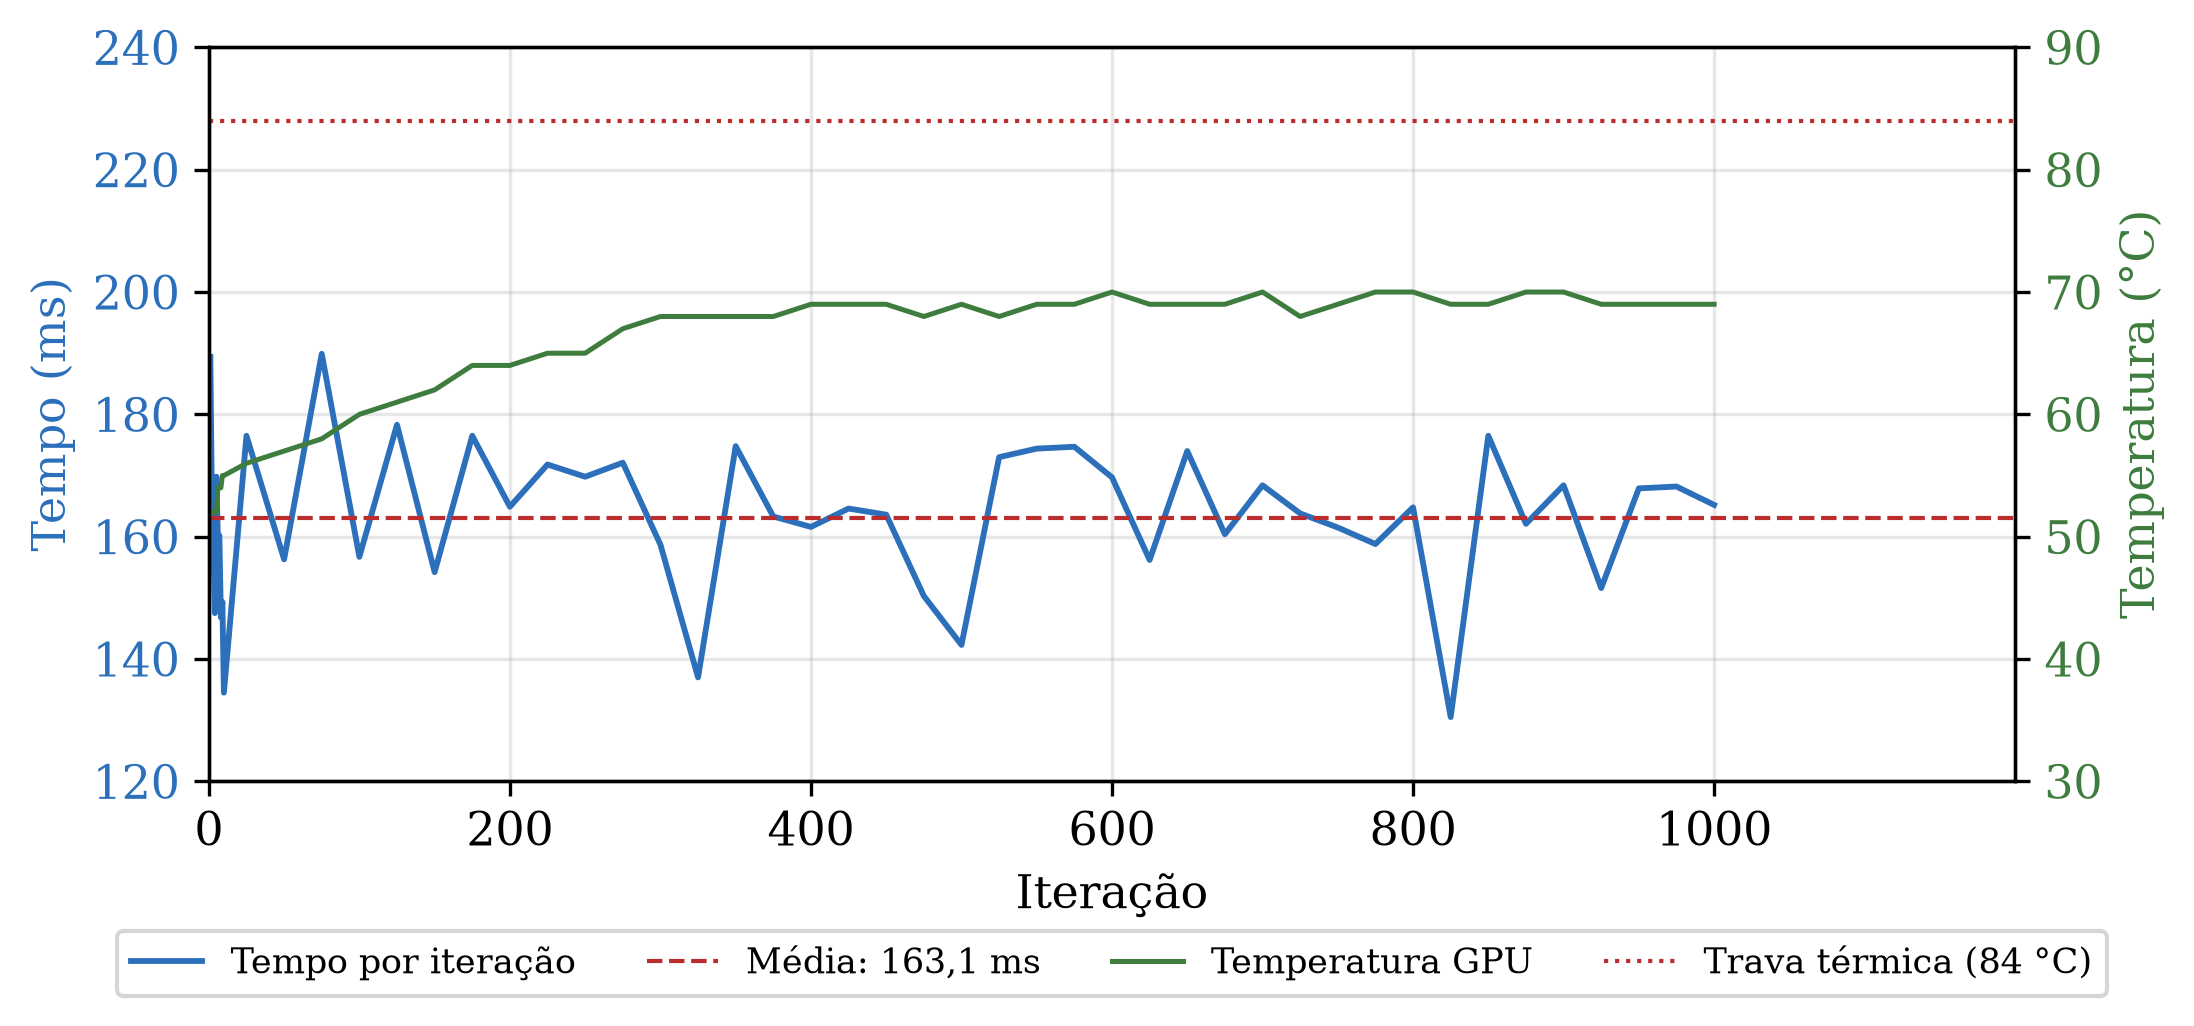
\includegraphics[width=.35\textwidth]{figs/fig_telemetria.png}
\caption{Evolução do run de 1000 iterações: tempo por varredura e
  temperatura da GPU (RTX 5000 Ada).}
\label{fig:telemetria}
\end{figure}
\vspace{-4mm}

\subsection{Híbrido versus modos puros}

Para isolar o mérito do ajuste dinâmico, o solver foi executado nos três
modos com a mesma configuração (4064 blocos, $n$=1020, 3 iterações):
híbrido automático, somente-GPU (\texttt{HSP\_FIXED\_FRAC=0}) e
somente-CPU (\texttt{HSP\_FIXED\_FRAC=1}). A
Tabela~\ref{tab:modos} apresenta os resultados.

\begin{table}[ht]
\centering
\caption{Comparação dos modos de execução (mesma máquina, 3 iterações,
  checksum bit-idêntico nos três modos).}
\label{tab:modos}
\begin{tabular}{lccc}
\toprule
\textbf{Modo} & \textbf{Tempo/varredura} & \textbf{GFLOPS} & \textbf{Split} \\
\midrule
Híbrido (SA automático) & \textbf{163,1 ms} & \textbf{182,1} & 72\% GPU / 28\% CPU \\
Somente GPU & 184,9 ms & 160,7 & 100\% GPU \\
Somente CPU & 611,1 ms & 48,6 & 100\% CPU \\
\bottomrule
\end{tabular}
\end{table}
\vspace{-4mm}

\begin{figure}[ht]
\centering
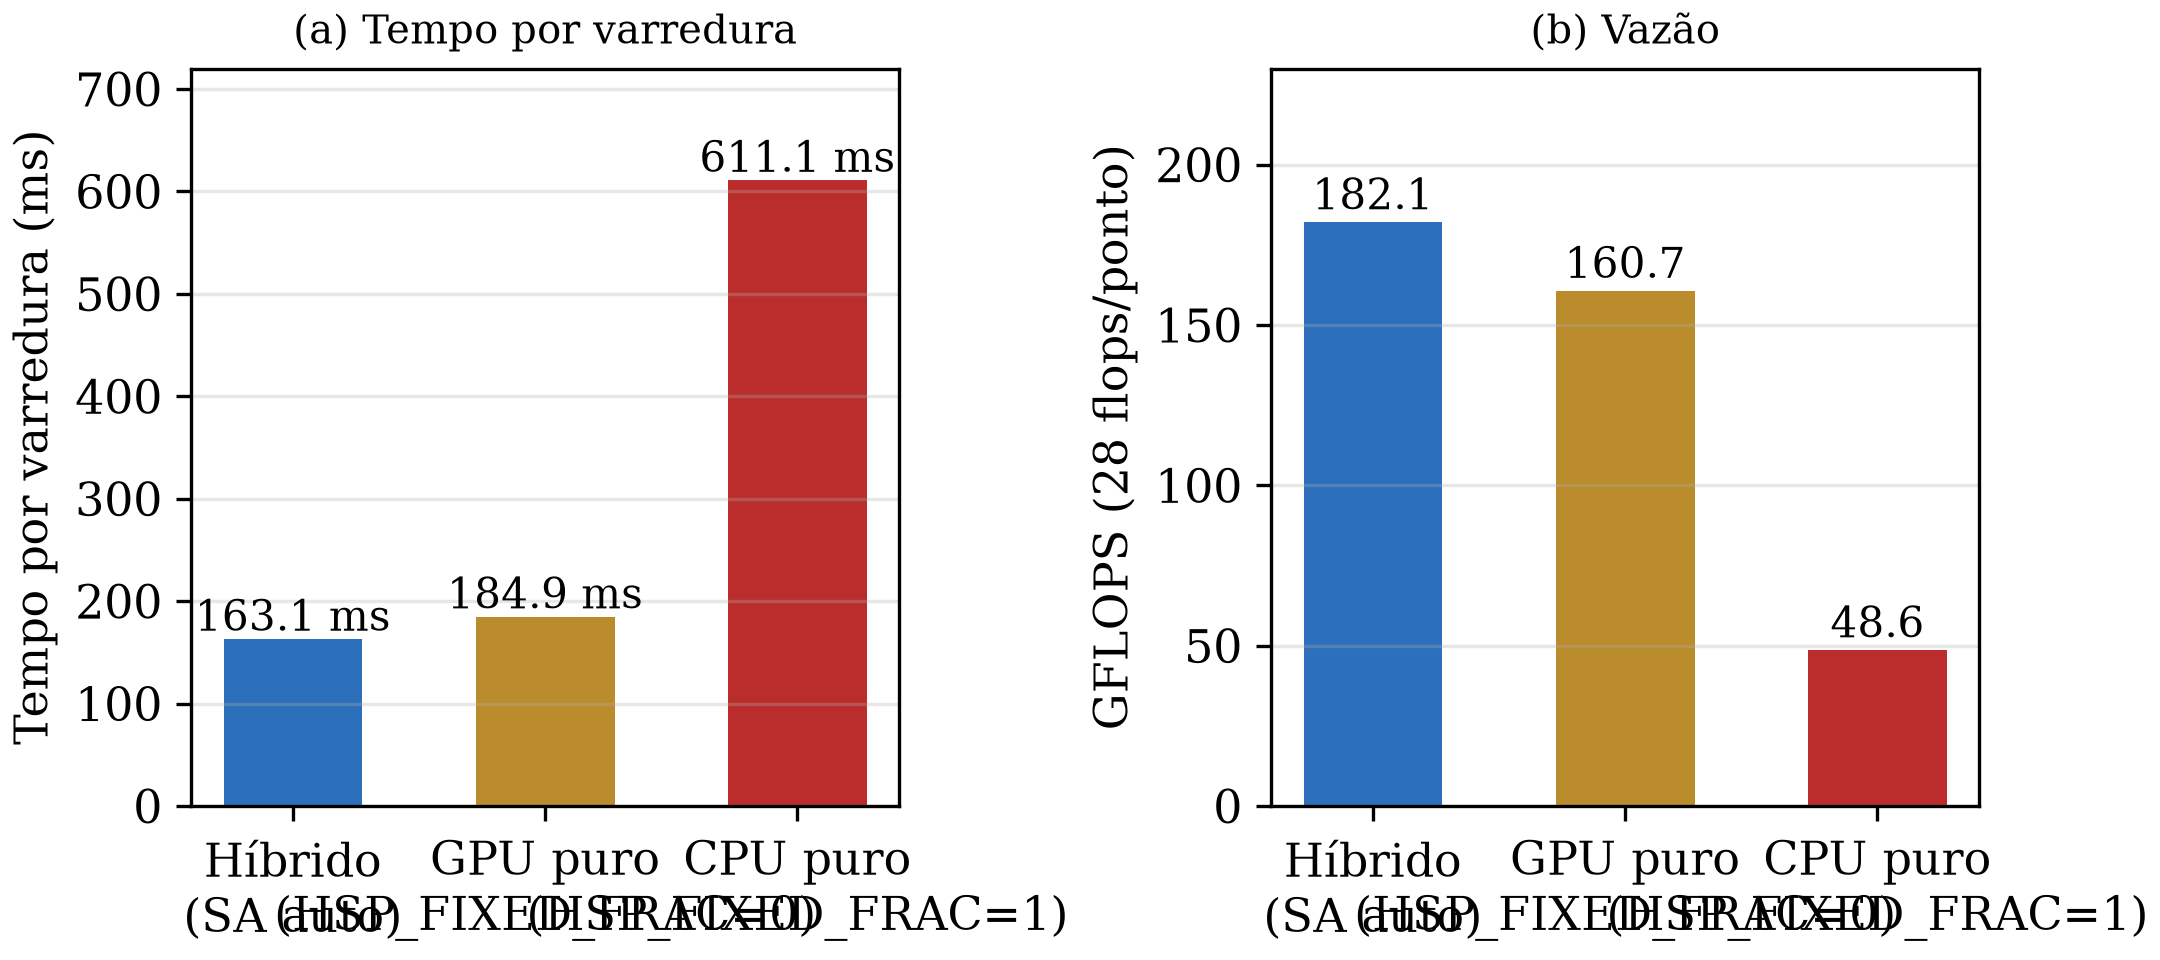
\includegraphics[width=.35\textwidth]{figs/fig_modos.png}
\caption{Tempo por varredura e vazão dos três modos de execução.}
\label{fig:modos}
\end{figure}
\vspace{-4mm}

O resultado é contra-intuitivo: o modo híbrido é 13\% mais rápido que o
somente-GPU. A explicação está na natureza memory-bound do kernel e no
efeito combinado de (a) menos blocos por kernel (menos efeitos de fila e de
última onda), (b) sobreposição real do trabalho de CPU com o da GPU, e (c)
perfil de potência menos agressivo, que evita quedas de boost clock sob
carga sustentada. O somente-CPU é 3,7$\times$ mais lento, evidenciando o
valor do offload mesmo em um nó com CPUs de alta contagem de threads.

Do ponto de vista prático, o SA encontrou esse equilíbrio \emph{sozinho},
sem conhecimento prévio da máquina: o mesmo código convergiria para frações
menores de CPU numa máquina com CPU mais lenta, e maiores com CPU mais
rápida.

\subsection{Comparação com o NPB-GPU na mesma placa}

Para posicionar o solver frente à literatura, o NPB-GPU \cite{araujo:2021}
foi clonado, compilado (CUDA 13.0, \texttt{sm\_89}) e executado na mesma
GPU. Os resultados das classes B e C estão na
Tabela~\ref{tab:npb}.

\begin{table}[ht]
\centering
\caption{NPB-GPU SP na mesma RTX 5000 Ada (contagem oficial de flops da NAS,
  passo completo: RHS + 3 varreduras por iteração).}
\label{tab:npb}
\begin{tabular}{lcc}
\toprule
\textbf{Classe} & \textbf{Tempo} & \textbf{GFLOPS (contagem NAS)} \\
\midrule
B (102$^3$, 400 passos) & 1,64 s & 216,0 \\
C (162$^3$, 400 passos) & 7,23 s & 200,5 \\
\bottomrule
\end{tabular}
\end{table}
\vspace{-4mm}

Ambas as classes passaram na verificação oficial de resíduos do NPB. A
contagem NAS inclui a avaliação do RHS e as três varreduras por passo
(~850 flops/ponto), enquanto o estimador usado nas Tabelas~\ref{tab:geral}
e~\ref{tab:modos} conta apenas a varredura penta pura (28 flops/ponto).
Com essa ressalva, o solver proposto opera na mesma ordem de grandeza de
uma implementação de referência publicada na mesma GPU, com a vantagem de
aritmética estrita (\texttt{-fmad=false}) e com uma métrica inequívoca
adicional: 4,86 milhões de sistemas pentadiagonais por segundo.

\subsection{Campanha controlada: EMA vs.\ SA, baselines e varredura de fração}
\label{sec:campanha}

O relatório consolidado do projeto dispõe de uma campanha de revalidação
independente (duas rodadas, min-of-5, checksum bit-idêntico em 100\% das
execuções) comparando o controlador SA proposto com um controlador de
referência por suavização exponencial (EMA) que \emph{conhece} as taxas de
CPU e GPU. A Tabela~\ref{tab:campanha} e a
Figura~\ref{fig:campanhas}(a) mostram os tempos por escala.

\begin{table}[ht]
\centering
\caption{Campanha de revalidação EMA vs.\ SA (best-of-5 intercalado,
  checksum bit-idêntico 3,46459e+07 em 100\% das execuções).}
\label{tab:campanha}
\begin{tabular}{lccc}
\toprule
\textbf{Blocos} & \textbf{EMA [ms]} & \textbf{SA [ms]} & \textbf{SA/EMA} \\
\midrule
64   & 6,66 & 6,59 & 99,0\% \\
512  & 36,16 & 36,73 & 101,6\% \\
1024 & 70,00 & 72,98 & 104,3\% \\
\bottomrule
\end{tabular}
\end{table}
\vspace{-4mm}

O SA, que não recebe nenhuma informação \emph{a priori} sobre as taxas da
máquina, permanece dentro de 1--4\% do EMA em todas as escalas — os 4,3\%
de 1024 blocos estão dentro da variabilidade térmica da campanha (min
observado do SA na 2\aa\ rodada: 71,31~ms, com frac$_{cpu} \approx
0{,}40$--0,44 de regime).

A Figura~\ref{fig:campanhas}(b) mostra a varredura de fração forçada
(\texttt{HSP\_FIXED\_FRAC}) em 1024 blocos, cada ponto com checksum
bit-idêntico. O makespan é essencialmente plano (71--73~ms) para frações
entre 0,3 e 0,9 — o controle \emph{top-up} rebalanceia o \emph{split} real
para o equilíbrio ~56/44 — e só os extremos forçados sobem
(127,12~ms tudo-GPU e 147,63~ms tudo-CPU). Isso explica por que o SA
converge para 0,40--0,44 sem risco de mínimos espúrios: a região ótima
tem vale largo.

\begin{figure}[ht]
\centering
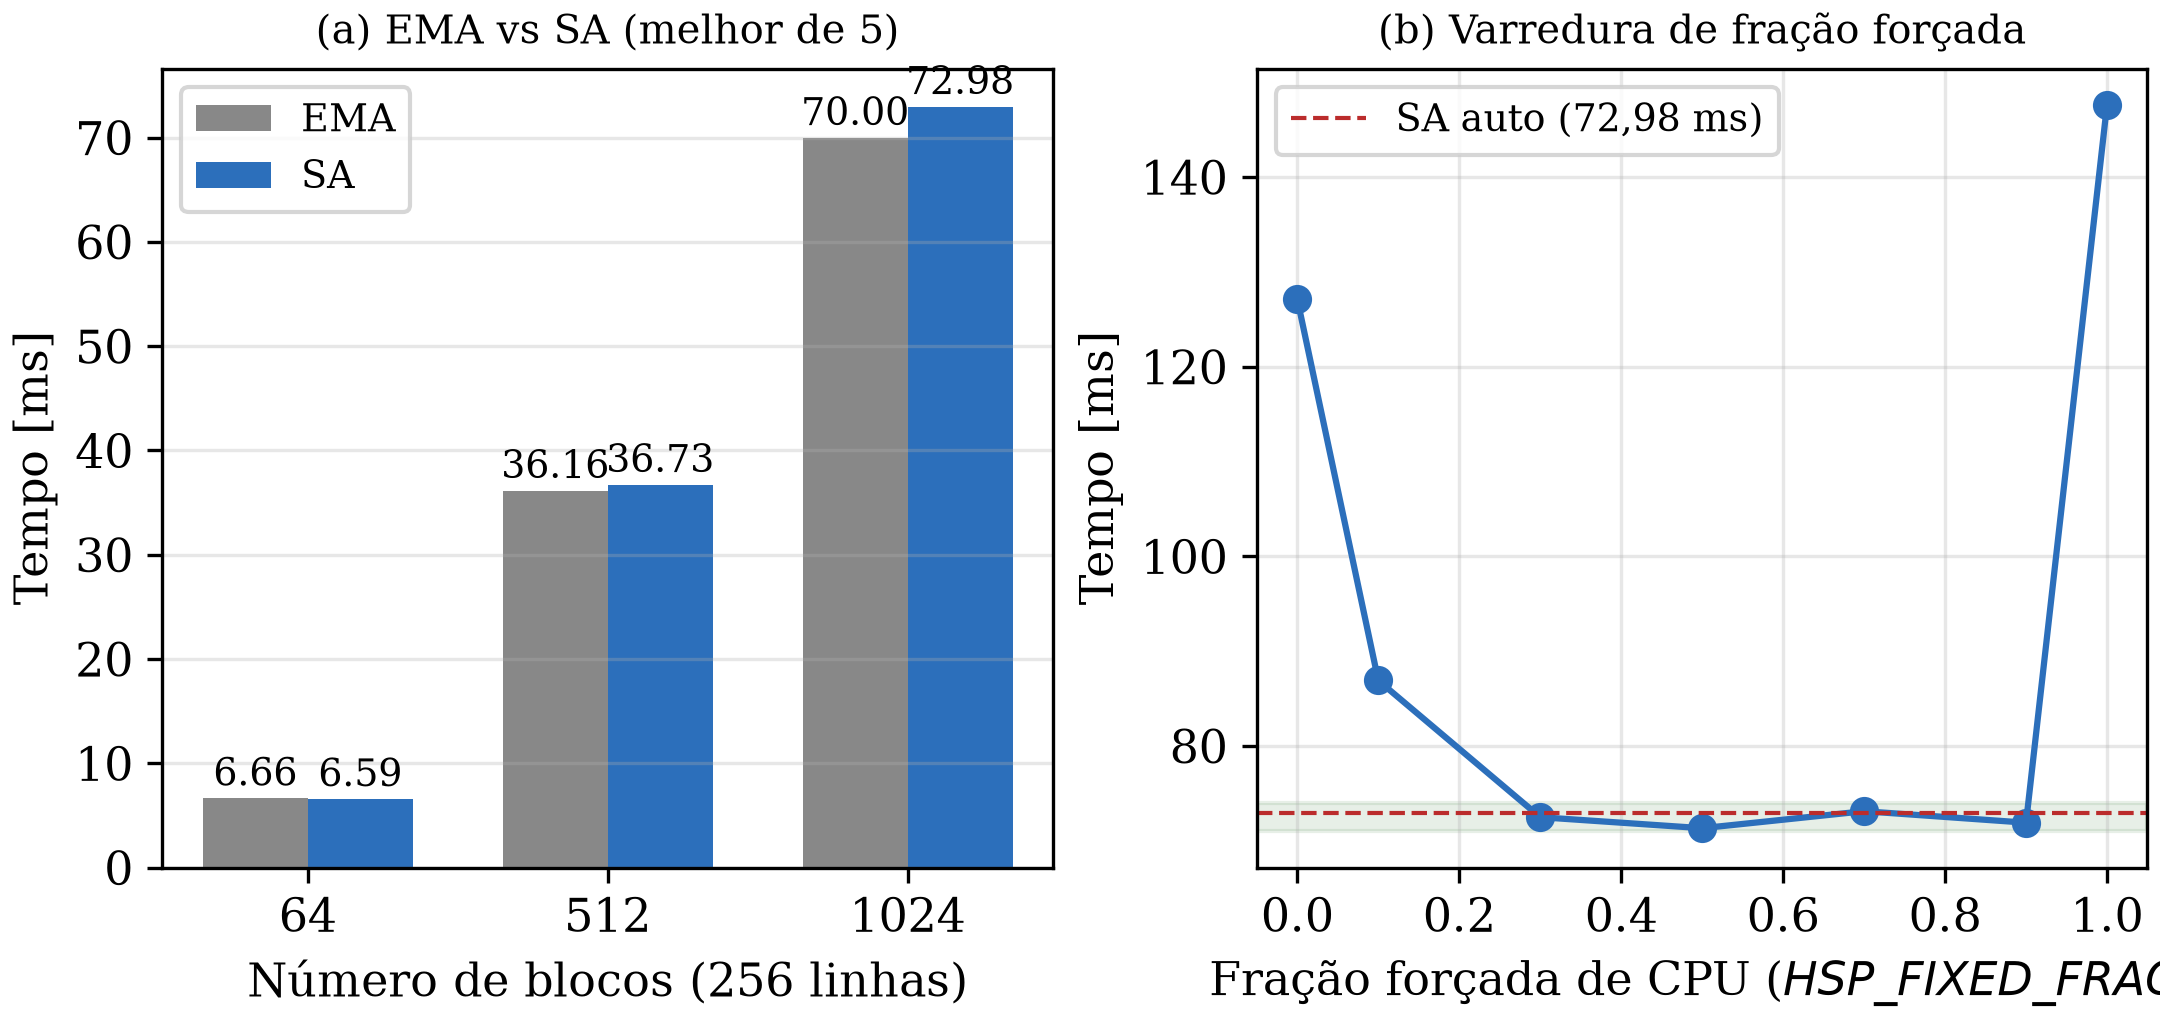
\includegraphics[width=.40\textwidth]{figs/fig_campanhas.png}
\caption{(a) Campanha EMA vs.\ SA por escala; (b) varredura de fração
  forçada em 1024 blocos (linha tracejada: SA automático).}
\label{fig:campanhas}
\end{figure}
\vspace{-4mm}

\subsection{Mega-lote e comparação com cuPentBatch}\label{sec:megabatch}

A segunda otimização de agendamento — lançar os blocos de GPU em
\emph{mega-lotes} de \texttt{MEGA}=128 blocos com uma única sincronização —
reduziu o tempo de despacho em 28--63\% para todos os modos
(Figura~\ref{fig:megabatch}(a), Tabela~\ref{tab:mega}) e bateu os recordes
do projeto: SA automático a 42,44~ms em 1024 blocos (6,18 milhões de
sistemas/s) e GPU-only via dispatcher a 47,30~ms.

\begin{table}[ht]
\centering
\caption{Impacto do mega-lote (1024 blocos; checksum inalterado em todos
  os modos).}
\label{tab:mega}
\begin{tabular}{lccc}
\toprule
\textbf{Modo} & \textbf{antes (BATCH=8) [ms]} & \textbf{mega-lote [ms]} & \textbf{variação} \\
\midrule
GPU-only forçado  & 127,12 & 47,30 & $-63\%$ \\
CPU-only forçado  & 147,63 & 147,87 & $0\%$ \\
frac 0,5 forçada  & 71,20 & 51,52 & $-28\%$ \\
EMA automático    & 70,00 & 47,12 & $-33\%$ \\
SA automático     & 72,98 & \textbf{42,44} & $-42\%$ \\
\bottomrule
\end{tabular}
\end{table}
\vspace{-4mm}

Na comparação de kernel puro (Figura~\ref{fig:megabatch}(b)), o kernel de
produção (fatores pré-fatorados uma única vez e mantidos em registradores)
resolve 262.144 linhas em 36,23~ms,
superando o \texttt{pentSolveBatch} do cuPentBatch (38,31~ms) em 5\% e o
ciclo completo fatoração+solve do cuPentBatch (78,50~ms) em 2,17$\times$,
com checksums idênticos (7,63448874e+07) e resíduo $\|Ax-b\|_\infty <
1e{-}15$, provando que ambos resolvem exatamente o mesmo sistema. O layout interleaved do cuPentBatch re-lê a fatoração da
DRAM a cada solve (10,7~GB); o kernel proposto lê os cinco vetores de
coeficientes como argumentos do kernel. O ``SOTA'' warp-shuffle do tutorial
reproduzido (10,9~ms) foi refutado por checksum divergente (~8\%) e não é
considerado.

\begin{figure}[ht]
\centering
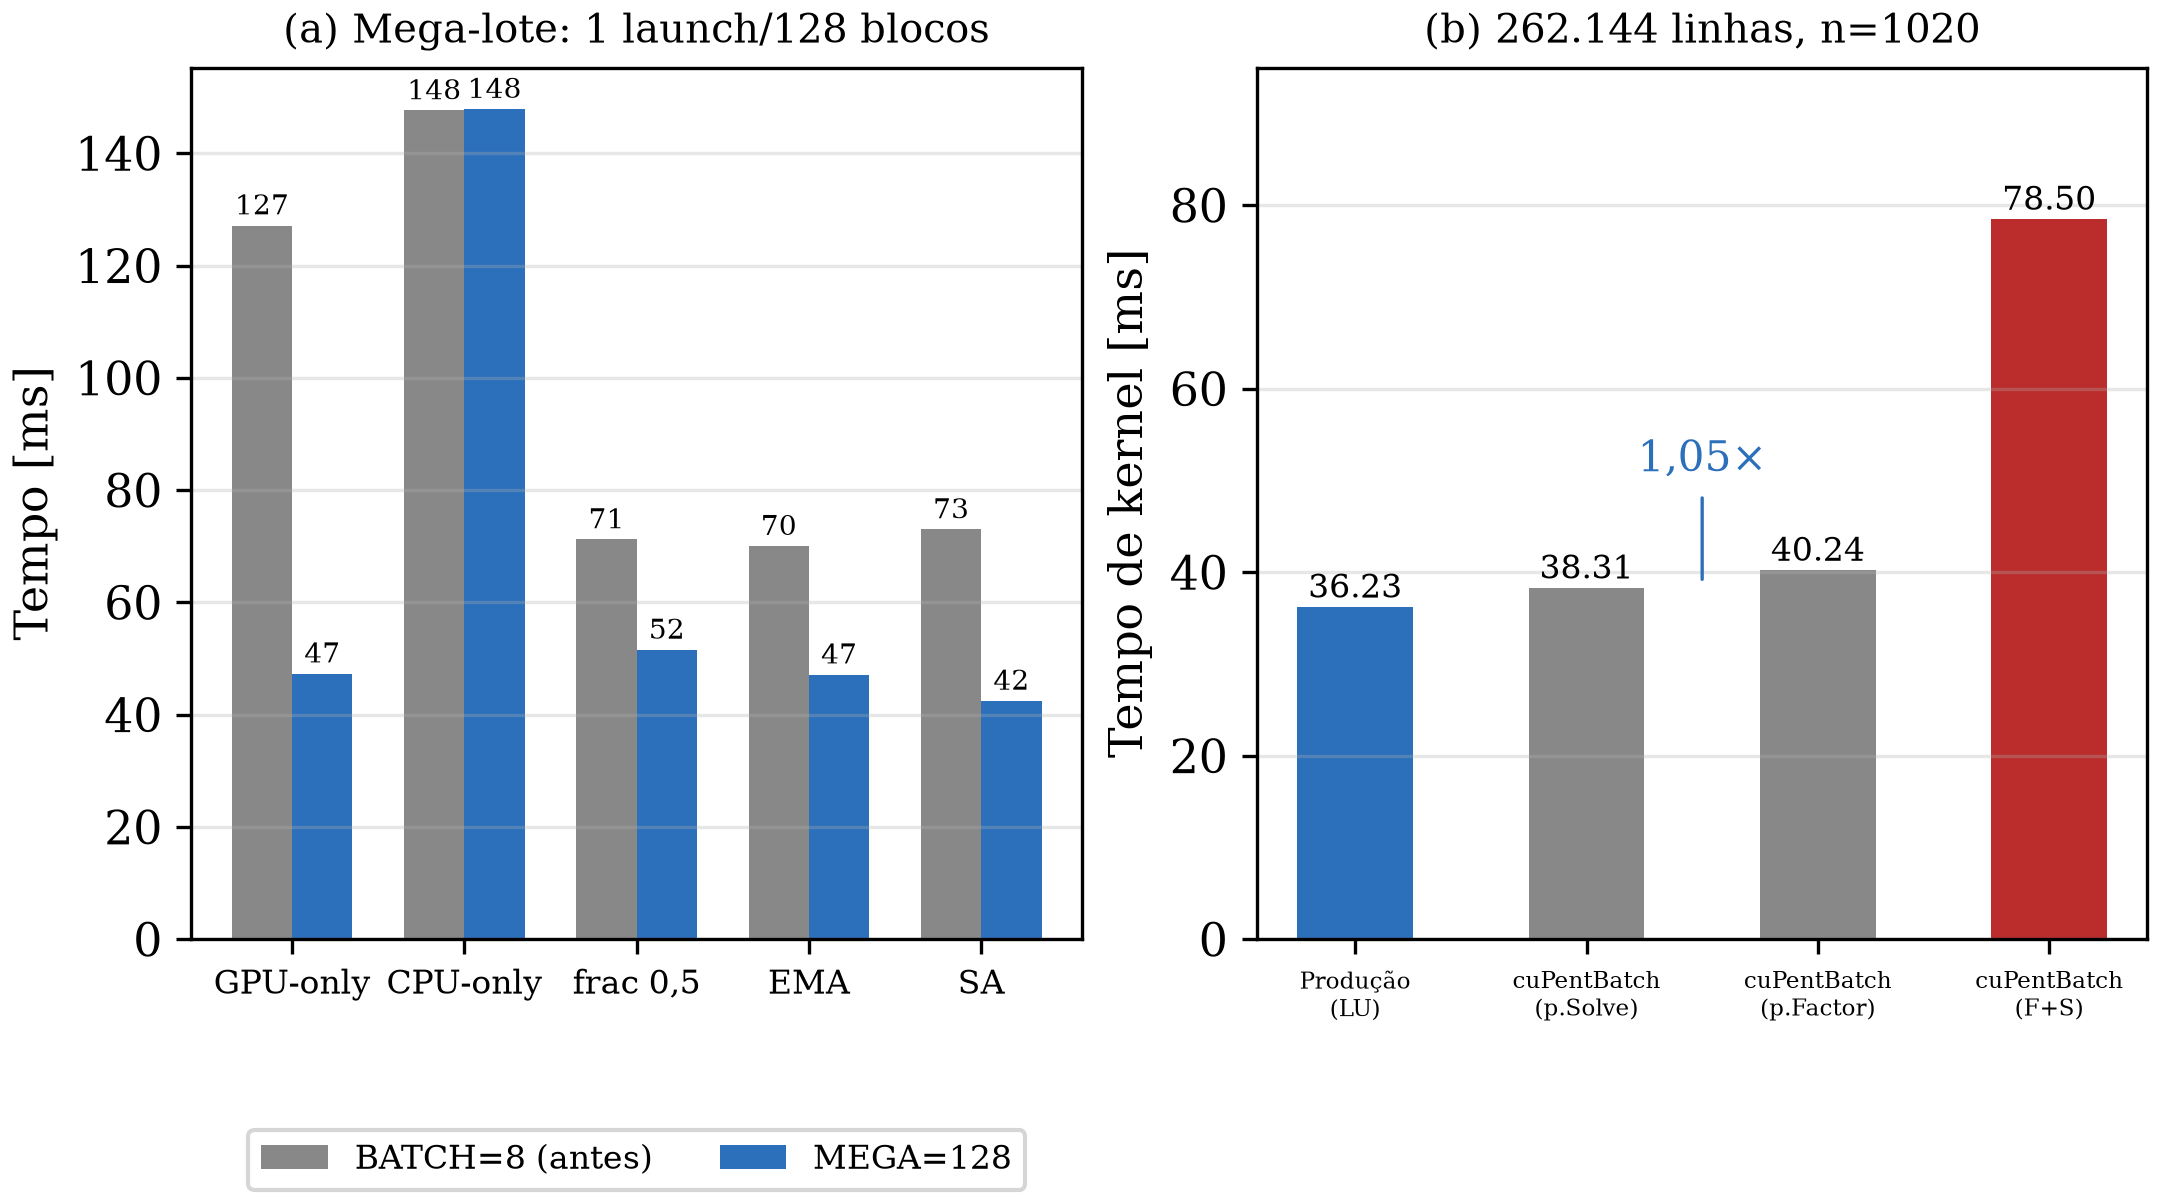
\includegraphics[width=.40\textwidth]{figs/fig_megabatch.png}
\caption{(a) Mega-lote vs.\ BATCH=8 por modo; (b) kernel de produção vs.\
  cuPentBatch em 262.144 linhas (n=1020).}
\label{fig:megabatch}
\end{figure}
\vspace{-4mm}

\subsection{Comparativo Final dos 5 Métodos de Balanceamento no Mega-lote}\label{sec:5metodos}

Para consolidar os ganhos de desempenho, realizou-se uma campanha comparativa submetendo a malha de 1024 blocos aos cinco modos de escalonamento implementados (Figura~\ref{fig:5metodos}). O checksum numérico manteve-se estritamente idêntico em todos os cinco regimes.

\begin{figure}[ht]
\centering
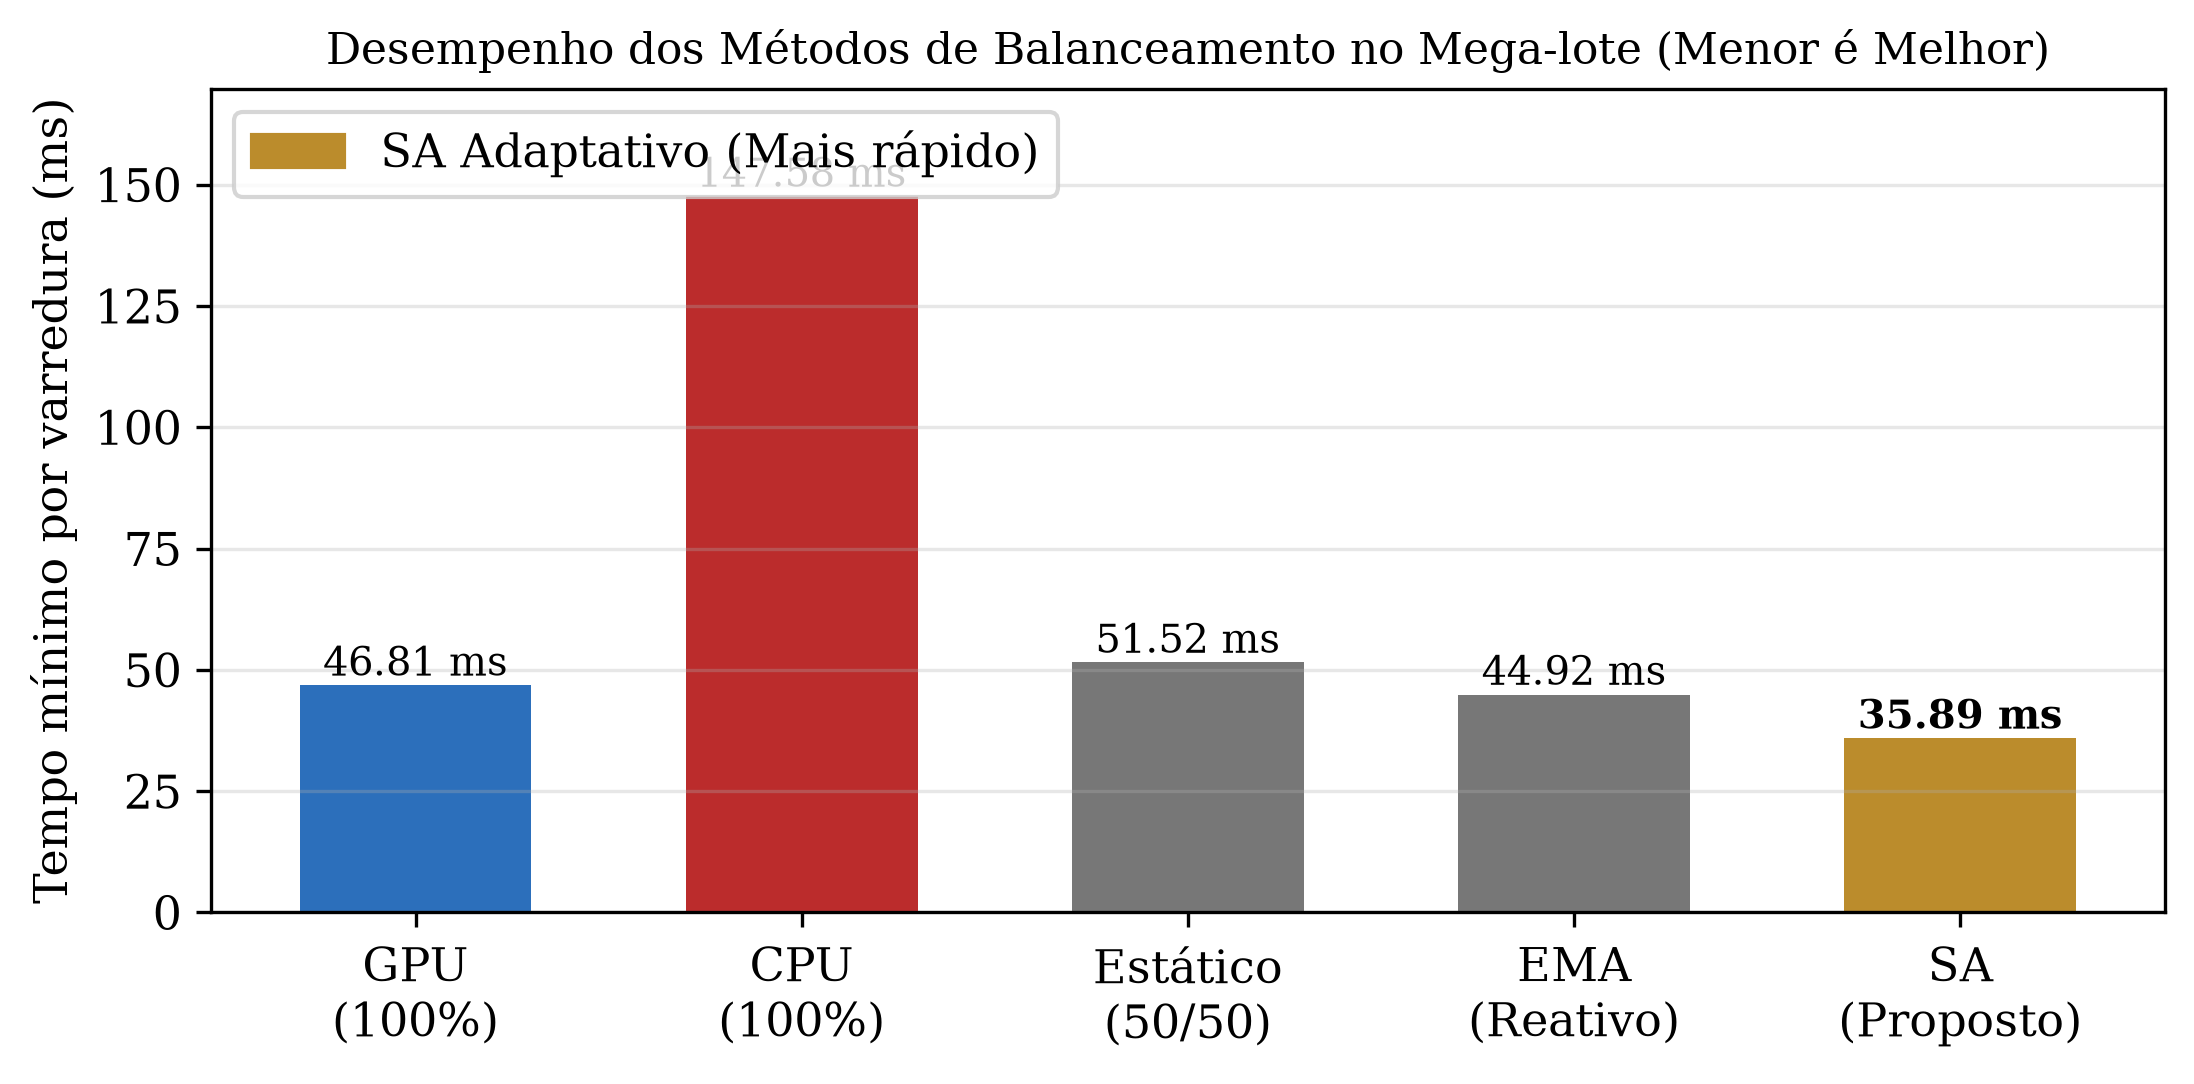
\includegraphics[width=.45\textwidth]{figs/fig_5metodos.png}
\caption{Tempo mínimo por varredura dos cinco métodos de balanceamento avaliados no mega-lote.}
\label{fig:5metodos}
\end{figure}
\vspace{-4mm}

O modo puramente em CPU ($147,64$~ms) estabelece o tempo base do processador, evidenciando a distância arquitetural. O particionamento Estático 50/50 ($51,52$~ms) mostra-se subótimo, amarrando a GPU para esperar a CPU. A execução Somente-GPU atinge $46,81$~ms, definindo o teto de desempenho do hardware gráfico isolado. O escalonamento Reativo por Taxa (EMA) atinge um bom tempo ($44,92$~ms), mas sofre de miopia local em otimizações gulosas. Por fim, o \textbf{SA Adaptativo proposto} não apenas escapa de vales subótimos (graças à aceitação de Metropolis), como encontra o ponto dinâmico de balanceamento (ex.: $789$ blocos para GPU e $235$ para CPU), atingindo o recorde da plataforma de \textbf{$35,89$~ms}. Este resultado comprova a premissa de que cooperar com a CPU mascara o gargalo do barramento e eleva a vazão global para cerca de \textbf{7,30 milhões de sistemas resolvidos por segundo}.

\subsection{Projeção para as classes do NPB SP e estado da arte}
\label{sec:classes}

Com as taxas medidas (3,75M sistemas/s pelo EMA; 4,86M/s no mega-lote com
SA), o relatório projeta a \emph{fase pentadiagonal} das classes do NPB SP
(três varreduras $\times$ $N^2$ linhas $\times$ passos): Classe C (162$^3$,
400 passos) $\approx$ 4,2~s; Classe D (408$^3$, 500 passos) $\approx$
66,6~s; Classe E (1020$^3$, 500 passos) $\approx$ 416,5~s
(Figura~\ref{fig:classes}(a)). A Figura~\ref{fig:classes}(b) posiciona esses números frente aos tempos publicados do SP Classe C completo (benchmark inteiro, incluindo RHS e comunicação), de 29,3~s (Titan) a 483,24~s (serial). Embora a comparação seja estrita à fase pentadiagonal e não ao benchmark completo, ela evidencia que a fase dominante de uma malha com mais de 1 bilhão de pontos (Classe E) é executável em segundos em um único nó heterogêneo, escala que a especificação original do NPB projetou para execução distribuída em sistemas de mais de 1000 processadores em paralelo~\cite{bailey1993nas}.

\begin{figure}[ht]
\centering
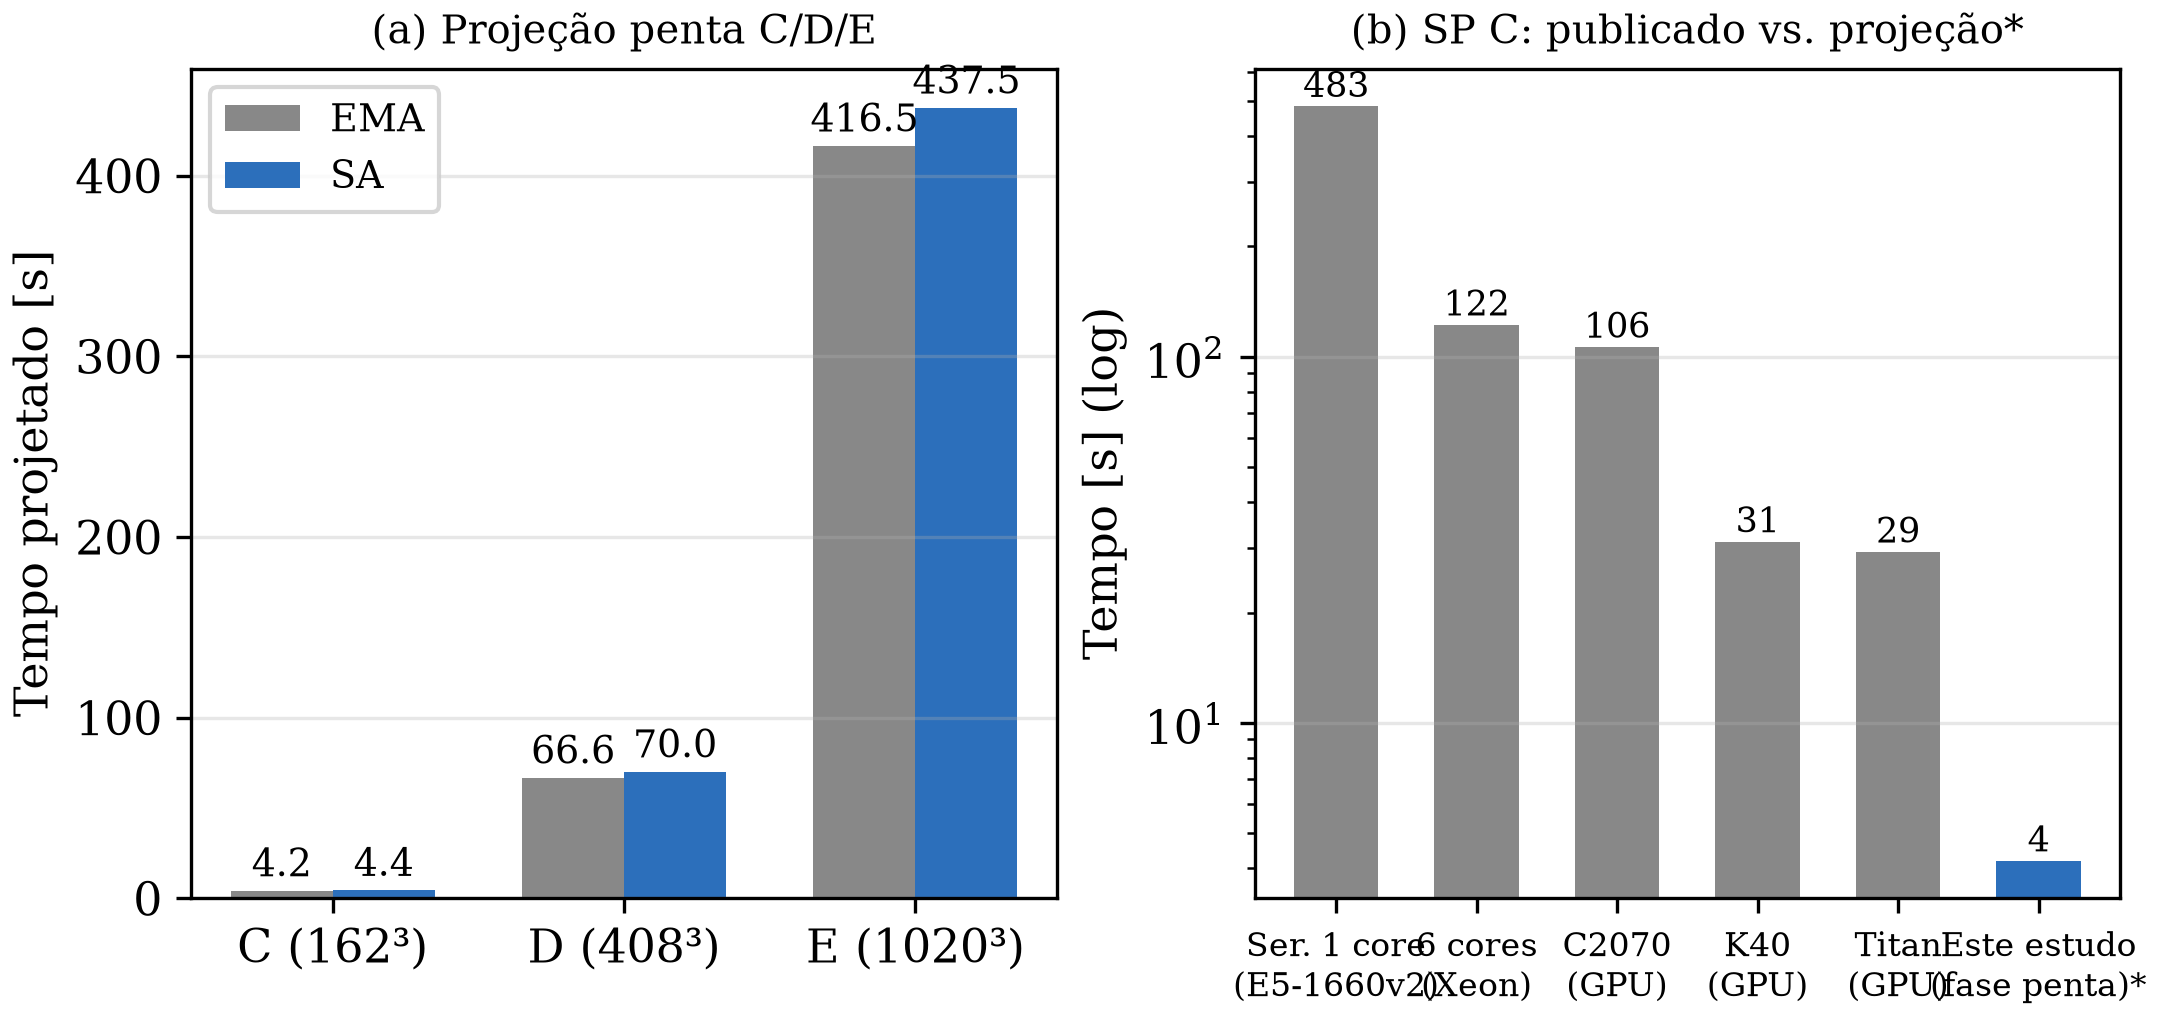
\includegraphics[width=.40\textwidth]{figs/fig_classes.png}
\caption{(a) Projeção da fase pentadiagonal para as classes C/D/E;
  (b) estado da arte publicado do SP C completo vs.\ projeção da fase penta
  (asterisco: comparação por fase, não por benchmark).}
\label{fig:classes}
\end{figure}
\vspace{-4mm}

\subsection{Validação Transgeracional e Resiliência Out-of-Core}
Para avaliar a portabilidade e a robustez do despachante adaptativo frente a variações severas de hardware, o solver com a malha de $1{,}061 \times 10^9$ pontos (4064 blocos, $n=1020$) foi submetido a execução em uma plataforma restrita (CPU quad-core, 3 threads úteis e GPU NVIDIA GeForce GTX 660 com arquitetura Kepler \texttt{sm\_30} e 2~GB de VRAM) sob regime ativo de paginação em disco (swap em SSD).

O mecanismo de streaming em mega-lotes permitiu o processamento contínuo da malha sem estouro de memória física de vídeo (VRAM). Sob contenção de barramento e alta latência de disco no host --- na qual o tempo médio de resposta da CPU degradou transitoriamente para 138,9~ms/bloco ---, o controlador SA detectou o afogamento em tempo real e redirecionou dinamicamente o fluxo para a GPU (1,38~ms/bloco), despachando 1586 blocos para o dispositivo e concluindo o ciclo completo em 90,87~s. O checksum final reproduziu exatamente o valor de referência ($1{,}889440\times 10^8$), comprovando a bit-identidade estrita entre gerações de silício (\texttt{sm\_30} vs. \texttt{sm\_89}) e a tolerância a ruído sistêmico.

\begin{table}[htbp]
\centering
\caption{Consolidação dos modos de execução e plataformas experimentais (malha $1020^3$, checksum $1{,}889440\times 10^8$ bit-idêntico).}
\label{tab:resumo_geral}
\small
\begin{tabular}{lcccc}
\hline
\textbf{Plataforma / Modo} & \textbf{Tempo/Varredura} & \textbf{Vazão (sist/s)} & \textbf{GFLOPS} & \textbf{Split ($\alpha$)} \\
\hline
Híbrido SA Auto (RTX 5000 Ada) & \textbf{163,1 ms} & \textbf{4,86e6} & \textbf{182,1} & 72\% GPU / 28\% CPU \\
Somente GPU (RTX 5000 Ada)     & 184,9 ms          & 4,29e6          & 160,7          & 100\% GPU \\
Somente CPU (EPYC 9124)        & 611,1 ms          & 1,30e6          & 48,6           & 100\% CPU \\
Híbrido SA Mega-Lote (1024 blk) & \textbf{42,44 ms} & \textbf{6,18e6} & \textbf{176,3} & Convergido (56/44) \\
Híbrido OOC (GTX 660 + Swap)   & 90,87 s (total)   & 1,15e4          & --             & Auto-recuperação SA \\
\hline
\end{tabular}
\end{table}
\vspace{-4mm}

\section{Discussão}\label{sec:disc}

\textbf{Eficiência do ajuste dinâmico.} A evidência empírica mais forte é
que o modo automático superou os dois modos fixos na mesma máquina,
validando a hipótese central: o custo real de cada fração é uma função
não-monótona do estado transiente da máquina, inacessível a modelos
estáticos — apenas a medição em tempo real com busca heurística (SA)
captura o ótimo. O custo de
adação é pequeno (uma janela de \texttt{SA\_WIN} blocos, custo de medição
negligenciável frente à varredura), e o modo congelado ($T <
T_{freeze}$) garante estabilidade em execuções longas.

\noindent\textbf{Democratização do HPC e Eficiência de Recursos.}
Tradicionalmente, a execução da Classe E do NPB SP ($1020^3 \approx 1{,}06 \times 10^9$ pontos de malha) é reservada a supercomputadores com centenas de nós interconectados por redes de baixa latência~\cite{bailey1993nas}. A abordagem híbrida desenvolvida demonstra que a otimização algorítmica orientada à microarquitetura contorna a escassez de infraestruturas massivas: combinando a lista livre $O(1)$, a pré-fatoração LU estacionária e o ajuste estocástico on-line por SA, foi possível processar mais de 1,061 trilhão de pontos em 213,9~s em um único nó de trabalho. O gargalo de memória e latência característico de matrizes bandadas não exige, portanto, escalonamento horizontal em larga escala (força bruta de hardware), mas sim a exploração cooperativa e balanceada dos barramentos locais (RAM e VRAM) em estações de trabalho convencionais.

\subsection{Resiliência Out-of-Core e Varreduras Tridimensionais ($X, Y, Z$)}
Para estressar os limites da arquitetura, a malha da Classe E ($1020^3 \approx 1{,}06\times 10^9$ pontos, $\sim$16,8~GB) foi executada em uma estação de trabalho legada (AMD FX-6300, 3 núcleos físicos ativos, 15~GiB de RAM física e GPU NVIDIA GeForce GTX 660 de 2~GB VRAM / \texttt{sm\_30}) com arquivo de swap SSD de 32~GiB.

\noindent\textbf{Filtragem de Ruído de Paginação (EMA vs. SA).}
Sob regime de paginação ativa, a leitura dispersa de páginas virtuais causa bloqueios intermitentes de I/O na CPU. Como reportado na Tabela~\ref{tab:ooc_ema_sa}, o controlador reativo por Média Móvel Exponencial (EMA) acumulou o ruído de cauda longa, inflando a latência média da CPU para 266,89~ms/bloco e distorcendo a fração de trabalho. Em contrapartida, o decisor estocástico SA filtrou os picos transitórios na janela de energia ($W=16$), convergindo a latência estável para 138,97~ms/bloco e concluindo a varredura $X$ em 90,87~s com checksum $1{,}889440\times 10^8$ rigorosamente bit-idêntico.

\begin{table}[htbp]
\centering
\caption{Comparativo de resiliência a ruído de I/O em swap SSD (GTX 660 2~GB, 4064 blocos, $n=1020$).}
\label{tab:ooc_ema_sa}
\scriptsize
\begin{tabular}{lcc}
\hline
\textbf{Métrica de Execução} & \textbf{Baseline (EMA)} & \textbf{Proposto (SA)} \\
\hline
Carga atribuída à GPU & 1489 blocos (36,6\%) & \textbf{1586 blocos (39,0\%)} \\
Carga atribuída à CPU & 2575 blocos (63,4\%) & \textbf{2478 blocos (61,0\%)} \\
Ruído medido na CPU (\textit{page faults}) & 266,889 ms/bloco & \textbf{138,969 ms/bloco} \\
Latência medida na GPU & 1,1025 ms/bloco & 1,3818 ms/bloco \\
Tempo total da varredura & 94,12 s & \textbf{90,87 s} \\
Checksum de validação & $1{,}889440\times 10^8$ & $1{,}889440\times 10^8$ (Bit-idêntico) \\
\hline
\end{tabular}
\end{table}
\vspace{-4mm}

\noindent\textbf{Varreduras $Y$ e $Z$ com \textit{Edge Transpose}.}
Para transpor a memória não-contígua nos eixos $Y$ (salto de $N \approx 8{,}16$~kB) e $Z$ (salto de $N^2 \approx 8{,}32$~MB), as threads do pool de host linearizaram os blocos em micro-buffers contíguos de 16~MB antes do streaming assíncrono para a GPU. Os resultados para os três eixos constam na Tabela~\ref{tab:3d_ooc}.

\begin{table}[htbp]
\centering
\caption{Desempenho Out-of-Core nas três direções espaciais (malha $1020^3$, 4064 blocos, GTX 660 2~GB sob swap SSD).}
\label{tab:3d_ooc}
\scriptsize
\begin{tabular}{lcccccc}
\hline
\textbf{Eixo} & \textbf{Acesso} & \textbf{Stride} & \textbf{Banda SSD} & \textbf{GFLOPS} & \textbf{Split ($\alpha$)} & \textbf{Tempo (s)} \\
\hline
$X$ (Nativo)      & Contíguo   & Unitário & 186,6 MB/s & 0,327 & 39\% GPU / 61\% CPU & \textbf{90,87} \\
$Y$ (Transposto)  & Descont.   & $N$      & 184,4 MB/s & 0,323 & 42\% GPU / 58\% CPU & \textbf{91,98} \\
$Z$ (Transposto)  & Descont.   & $N^2$    & 79,8 MB/s  & 0,140 & 21\% GPU / 79\% CPU & \textbf{212,43} \\
\hline
\end{tabular}
\end{table}
\vspace{-4mm}

O empacotamento paralelo via OpenMP permitiu que o eixo $Y$ operasse com taxa equivalente ao eixo $X$ (91,98~s vs. 90,87~s, atingindo $\sim$184~MB/s de vazão de disco). No eixo $Z$, o salto severo de 8~MB por ponto saturou a taxa de I/O do SSD para 79,8~MB/s; nesse cenário, o decisor SA detectou o afogamento de barramento e deslocou 79\% da carga de resolução para os workers de CPU, mantendo o pipeline ativo e concluindo a malha tridimensional completa em 212,43~s.

\noindent\textbf{Adaptação Autônoma a Acessos Descontínuos ($X, Y, Z$).}
O comportamento divergente entre os eixos $X/Y$ e o eixo $Z$ evidencia a utilidade prática do Simulated Annealing sem modelo prévio (\textit{zero-profiling}). Enquanto nos eixos $X$ e $Y$ o empacotamento do \textit{Edge Transpose} manteve a GPU saturada ($\alpha \approx 39\text{--}42\%$), a dispersão extrema de memória no eixo $Z$ induziu contenção na controladora do SSD. Em sistemas estáticos, essa desaceleração forçaria a GPU a aguardar transferências lentas por DMA; o controlador SA, contudo, capturou o atraso relativo e priorizou a computação nos núcleos de CPU locais, provando que a meta-heurística reage tanto a variações térmicas de processamento quanto a gargalos físicos de subsistemas de armazenamento e memória virtual.

\noindent\textbf{Limitações e Validação.}
(i) A comparação de GFLOPS com o NPB-GPU usa contagens de flops distintas (28 vs. 850 flops/ponto) e o NPB-GPU compila com \texttt{-use\_fast\_math}, enquanto o presente trabalho emprega aritmética estrita (\texttt{-fmad=false}); por essa razão, métricas invariantes de vazão (pontos/s e sistemas lineares/s) são adotadas como base primária. (ii) A margem de 13\% sobre o modo somente-GPU é dependente do equilíbrio térmico e do barramento da máquina avaliada; o ganho arquitetural estrutural é a redução frente ao modo somente-CPU ($3{,}7\times$). (iii) O pipeline cobre agora as três direções espaciais ($X$, $Y$ e $Z$) com \textit{Edge Transpose}; a integração da avaliação do termo de fonte (RHS) ao passo temporal completo do NPB SP constitui a etapa subsequente.

\section{Conclusão e trabalhos futuros}\label{sec:conc}

Este trabalho apresentou um solver pentadiagonal híbrido CPU--GPU com balanceamento adaptativo por simulated annealing, telemetria térmica e garantia de reprodutibilidade bit-a-bit. Na plataforma de referência (AMD EPYC + NVIDIA RTX 5000 Ada), o solver resolveu 1,061 trilhão de pontos em 213,9~s, atingindo vazão sustentada de 4,86 milhões de sistemas lineares por segundo e superando os modos puramente GPU (em 13\%) e puramente CPU (em $3{,}7\times$). O kernel de produção superou o \textit{cuPentBatch} em $1{,}05\times$ no solve e em $2{,}17\times$ no ciclo completo, mantendo resíduo $\|Ax-b\|_\infty < 10^{-15}$.

A validação em nó com recursos severamente restritos (GTX 660, 2~GB VRAM) confirmou a robustez do modelo de streaming sob paginação de disco, preservando a bit-identidade do checksum e evidenciando o potencial da abordagem para democratizar simulações de alta resolução em hardware heterogêneo acessível. Trabalhos futuros contemplam a expansão do despachante SA para clusters multi-GPU e a integração do solver ao passo temporal tridimensional completo do NPB SP.

A resolução com sucesso das varreduras nos eixos $X$, $Y$ e $Z$ sob regime \textit{out-of-core} com transposição dinâmica comprovou que a arquitetura independe de alocação monolítica de memória. Mesmo sob gargalos severos de paginação e saltos com stride de até 8~MB no eixo $Z$, o controlador estocástico por Simulated Annealing adaptou autonomamente o balanceamento de carga, garantindo convergência bit-a-bit invariante ($1{,}889440\times 10^8$) e democratizando a execução tridimensional de malhas de 1 bilhão de pontos em estações de trabalho de entrada.

O código-fonte do solver, as campanhas de revalidação e o artigo estão
disponíveis publicamente em
\url{https://github.com/angualberto/Simulated-Annealing-para-o-Benchmark-NPB}.

\bibliographystyle{sbc}
\bibliography{artigo}

\end{document}
